\documentclass[a4paper]{article}

\usepackage[a4paper,margin=2cm]{geometry}
\usepackage{amsmath}
\usepackage{graphicx}
\usepackage[table]{xcolor}
\usepackage{tikz}
\usepackage{minted}
\usepackage[clock]{ifsym}
\usepackage{subcaption} % subfigures
\usepackage{hyperref} % links in table of contents
\usepackage[strings]{underscore}

\usetikzlibrary{calc,positioning,shapes,arrows.meta,decorations.pathreplacing}
\graphicspath{ {./graphics/} }

\hypersetup{
	colorlinks,
	citecolor=black,
	filecolor=black,
	linkcolor=black,
	urlcolor=black
}
\numberwithin{figure}{section}
\numberwithin{table}{section}
\renewcommand{\arraystretch}{1.5}

\newcommand{\mi}{\mintinline}
\newcommand{\NA}{---}

\title{CS2022 - Project 2}
\date{2019-04-14}
\author{\url{https://git.nul.ie/dev/cs2022}\\\url{https://github.com/devplayer0/cs2022}\\Jack O'Sullivan\\\href{mailto:osullj19@tcd.ie}{osullj19@tcd.ie}\\17331147}

\begin{document}
\maketitle
\tableofcontents
\pagenumbering{gobble}

\newpage
\pagenumbering{arabic}
\section{Introduction}
The goal of this assignment was to complete a functional microprogrammed processor, implementing a number of intructions.

\section{Testbench results}
This section details results of the testbenches for the components created in project 2.

\subsection{\mi{c}{memory}}
\begin{figure}[h!]
	\centering
	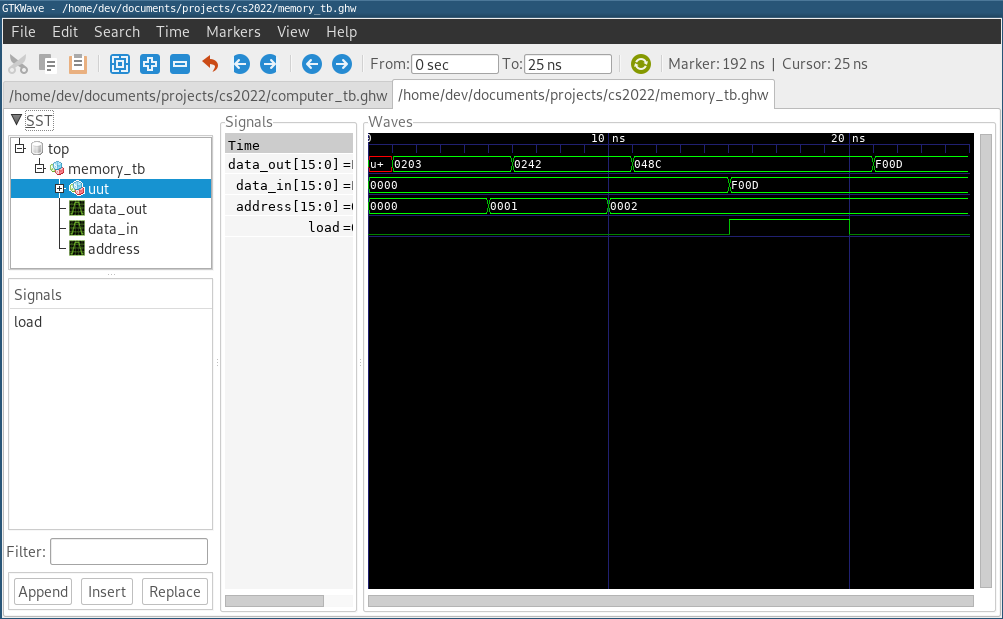
\includegraphics[width=\textwidth]{memory_tb}
	\caption{\mi{c}{memory} testbench results}
	\label{fig:memory}
\end{figure}

Figure~\ref{fig:memory} shows the simulation results of the 512x 16-bit word main memory.
\begin{itemize}
	\item After a short delay, setting the input address to \mi{c}{0} produces \mi{c}{0x203} (the first 
		instruction in memory) at \mi{c}{data_out}.
	\item Increasing the address shows the following instructions.
	\item Setting \mi{c}{data_in} and the load signal to high shows that the data at \mi{c}{0x2} is overwritten.
\end{itemize}

\newpage
\subsection{\mi{c}{control_memory}}
\begin{figure}[h!]
	\centering
	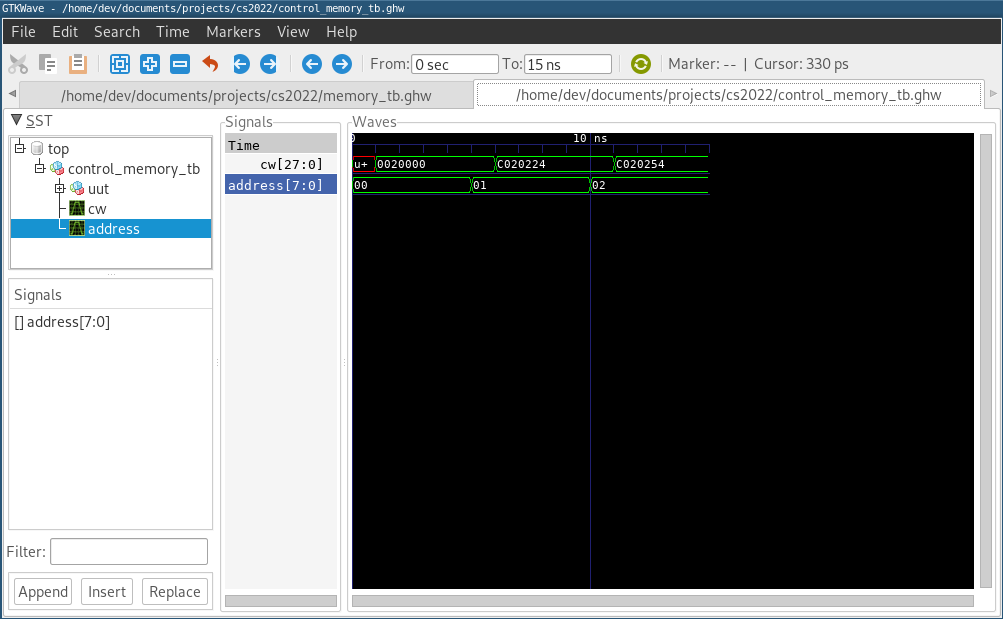
\includegraphics[width=\textwidth]{control_memory_tb}
	\caption{\mi{c}{control_memory} testbench results}
	\label{fig:cmemory}
\end{figure}

Figure~\ref{fig:cmemory} shows the simulation results of the 256x 28-bit word control (microcode) memory.

This memory just outputs the control word at the input address.

\newpage
\subsection{\mi{c}{flag_mux}}
\begin{figure}[h!]
	\centering
	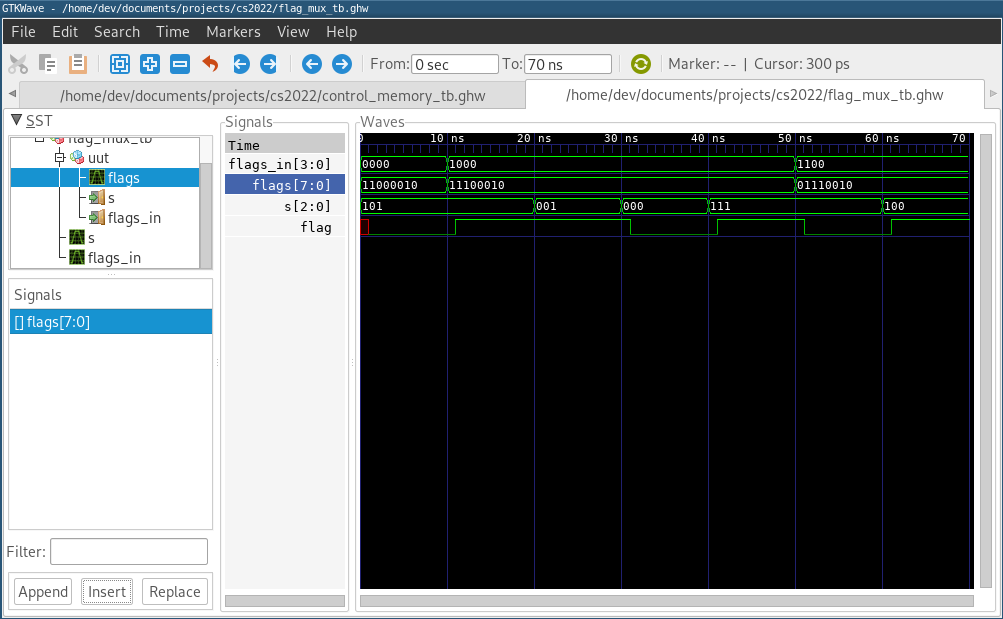
\includegraphics[width=\textwidth]{flag_mux_tb}
	\caption{\mi{c}{flag_mux} testbench results}
	\label{fig:fmux}
\end{figure}

Figure~\ref{fig:fmux} shows the simulation results of the flags mux, used to determine if the next CAR address 
should be loaded or incremented.

\mi{c}{flag} is the value of the bit selected from the internal \mi{c}{flags} vector by \mi{c}{s}.
\begin{itemize}
	\item \mi{vhdl}{flags(7) <= ~Z}
	\item \mi{vhdl}{flags(6) <= ~C}
	\item \mi{vhdl}{flags(5 downto 2) <= flags_in} (in the order \mi{c}{NZVC})
	\item \mi{vhdl}{flags(1) <= "1"} (constant)
	\item \mi{vhdl}{flags(0) <= "0"} (constant)
\end{itemize}

\newpage
\subsection{\mi{c}{car}}
\begin{figure}[h!]
	\centering
	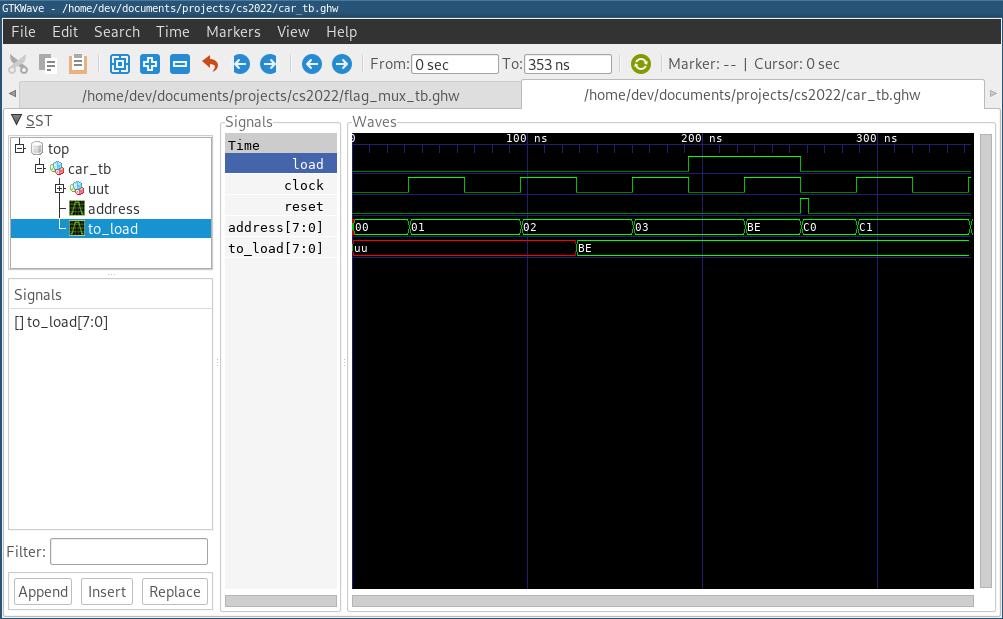
\includegraphics[width=\textwidth]{car_tb}
	\caption{\mi{c}{car} testbench results}
	\label{fig:car}
\end{figure}

Figure~\ref{fig:car} shows the simulation results of the Control Address Register (CAR).

\begin{itemize}
	\item When \mi{c}{load} is low, the CAR will increment its value by 1 on every clock.
		When high, it will load the input address on the next clock.
	\item Pulling \mi{c}{reset} high will set the address to \mi{c}{0xc0}, the address of the instruction fetch
		control word in the control memory.
\end{itemize}

\newpage
\subsection{\mi{c}{pc_extend}}
\begin{figure}[h!]
	\centering
	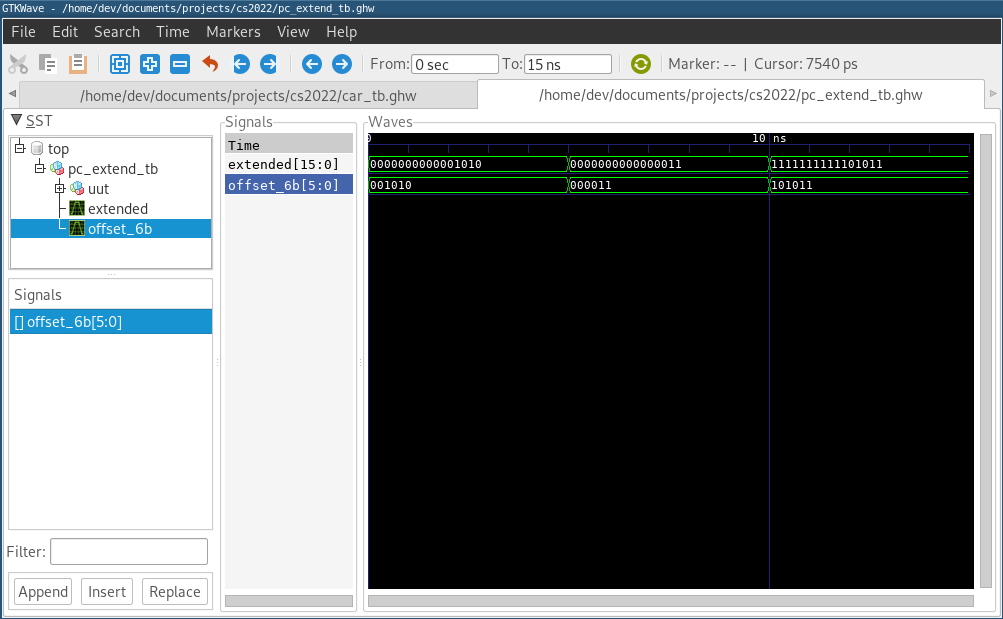
\includegraphics[width=\textwidth]{pc_extend_tb}
	\caption{\mi{c}{pc_extend} testbench results}
	\label{fig:pcext}
\end{figure}

Figure~\ref{fig:pcext} shows the simulation results of the Program Counter load extender.
This simply takes a 6 bit input (from the instruction register) and extends the top bit (sign) to 16 bits for 
input into the PC.

\newpage
\subsection{\mi{c}{pc}}
\begin{figure}[h!]
	\centering
	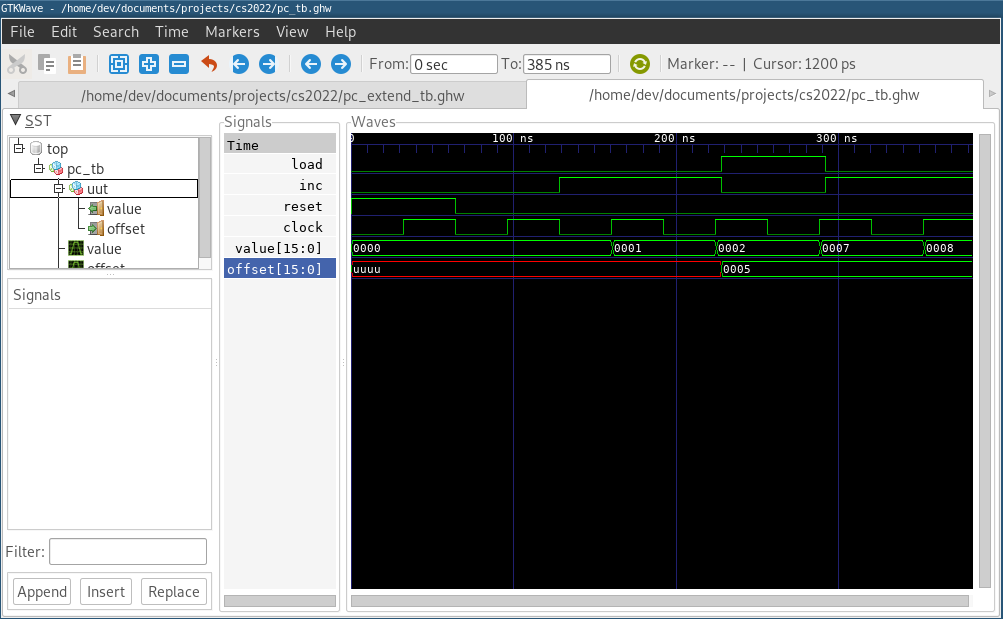
\includegraphics[width=\textwidth]{pc_tb}
	\caption{\mi{c}{pc} testbench results}
	\label{fig:pc}
\end{figure}

Figure~\ref{fig:pc} shows the simulation results of the Program Counter (PC).
\begin{itemize}
	\item When \mi{c}{inc} is high, the PC will increment its value on every clock.
	\item When \mi{c}{load} is high, the PC will add the input offset to its current value on the next clock.
\end{itemize}

\newpage
\section{Final processor}
This section will discuss the implemented instructions and results of the test program which utilises them.
\begin{figure}[h!]
	\centering
	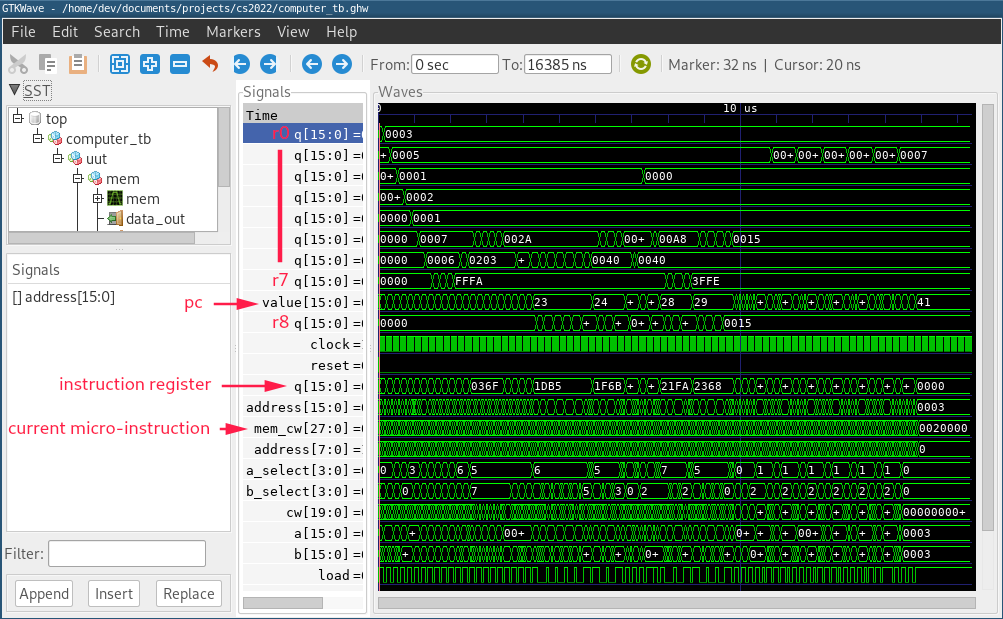
\includegraphics[width=\textwidth]{computer_overview}
	\caption{Complete processor testbench}
	\label{fig:coverview}
\end{figure}

\newpage
\subsection{Implemented instructions}
Below is a table of all of the implemented instructions and their corresponding opcodes and microcode words.
\begin{center}
\begin{tabular}{|l|l|l||l|}
	\hline
	\textbf{Opcode} & \textbf{Micro-op} & \textbf{Name} & \textbf{Description} \\
	\hline

	0   & \mi{vhdl}{x"0020000"} & \mi{c}{HLT} & halt (loop forever) \\
	1   & \mi{vhdl}{x"c020224"} & \mi{c}{ADI} & add immediate \\
	2   & \mi{vhdl}{x"c020254"} & \mi{c}{SUI} & subtract immediate \\
	3   & \mi{vhdl}{x"c020014"} & \mi{c}{INC} & increment register \\
	4   & \mi{vhdl}{x"c020064"} & \mi{c}{DEC} & decrement register \\
	5   & \mi{vhdl}{x"c020024"} & \mi{c}{ADD} & add registers \\
	6   & \mi{vhdl}{x"c020054"} & \mi{c}{SUB} & subtract registers \\
	7   & \mi{vhdl}{x"c020084"} & \mi{c}{AND} & logical \mi{c}{&} \\
	8   & \mi{vhdl}{x"c0200a4"} & \mi{c}{OR}  & logical \mi{c}{|} \\
	9   & \mi{vhdl}{x"c0200c4"} & \mi{c}{XOR} & logical \mi{c}{^} \\
	10  & \mi{vhdl}{x"c0200e4"} & \mi{c}{NOT} & logical \mi{c}{~} \\
	11  & \mi{vhdl}{x"c02000c"} & \mi{c}{LD}  & load from memory \\
	12  & \mi{vhdl}{x"c020001"} & \mi{c}{ST}  & store to memory \\
	13  & \mi{vhdl}{x"c020201"} & \mi{c}{STI} & store immediate to memory \\
	14  & \mi{vhdl}{x"8121004"} & \mi{c}{SLI} & shift left by immediate (stores source in r8), dst and a must be the same! \\
	15  & \mi{vhdl}{x"8021004"} & \mi{c}{SL}  & shift left by register (stores source in r8), dst and a must be the same! \\
	16  & \mi{vhdl}{x"8821004"} & \mi{c}{SRI} & shift right by immediate (stores source in r8), dst and a must be the same! \\
	17  & \mi{vhdl}{x"8721004"} & \mi{c}{SR}  & shift right by register (stores source in r8), dst and a must be the same! \\
	18  & \mi{vhdl}{x"c022000"} & \mi{c}{B}   & unconditional branch \\
	19  & \mi{vhdl}{x"8e20000"} & \mi{c}{BEQ} & branch if register is zero ("equal") \\
	127 & \mi{vhdl}{x"c020000"} & \mi{c}{NOP} & do nothing \\
	\hline
\end{tabular}
\end{center}

\smallskip
In order to fetch and execute the next instruction, there are two additional micro-ops towards the end of the 
control memory:

\begin{minted}[tabsize=4]{vhdl}
	192 =>		x"000c002", -- instruction fetch (and increment pc)
	193 =>		x"0030000", -- instruction execute
\end{minted}

\smallskip
Any locations in control memory not otherwise set are filled with \mi{vhdl}{x"002000"} (\mi{c}{HLT}) so that undefined opcodes stop the processor immediately:
\begin{minted}[tabsize=4]{vhdl}
	others =>	x"0020000"  -- go to halt instruction if unknown opcode
\end{minted}

\newpage
\smallskip
A few of the instructions (left / right shift and conditional branching) require additional microcode (note the next address portion of the control words above jumping to this additional code):
\begin{listing}[ht]
\begin{minted}[tabsize=4]{vhdl}
	-- left shift
	128 =>		x"8220104", -- copy the shift amount into dst (from register)
	129 =>		x"0000304", -- copy the shift amount into dst (from immediate)
	130 =>		x"8680000", -- is the shift amount (in a) equal to 0? if so, go to setting dst to r8. otherwise, continue.
	131 =>		x"0001584", -- shift r8 left by one
	132 =>		x"0000064", -- decrement a
	133 =>		x"8220000", -- goto checking shift done
	134 =>		x"c020804", -- set dst to r8 and goto IF

	-- right shift
	135 =>		x"8920104", -- copy the shift amount into dst (from register)
	136 =>		x"0000304", -- copy the shift amount into dst (from immediate)
	137 =>		x"8d80000", -- is the shift amount (in a) equal to 0? if so, go to setting dst to r8. otherwise, continue.
	138 =>		x"0001544", -- shift r8 right by one
	139 =>		x"0000064", -- decrement a
	140 =>		x"8920000", -- goto checking shift done
	141 =>		x"c020804", -- set dst to r8 and goto IF

	-- beq
	142 =>		x"1280000", -- goto unconditional branch if zero
	143 =>		x"c020000", -- otherwise continue as normal
\end{minted}
\label{label:extramc}
\end{listing}


\newpage
\subsection{Test program}
Below is the sample program as initialized into the start of memory. An ARM-like assembler syntax is used.
\begin{minted}{vhdl}
x"0203", -- adi r0, r0, 3
x"0242", -- adi r1, r0, 2
x"048c", -- sui r2, r1, 4
x"06d0", -- inc r3, r2
x"0918", -- dec r4, r3
x"0b59", -- add r5, r3, r1
x"0daa", -- sub r6, r5, r2
x"0fdd", -- and r7, r3, r5 ; (2 & 7)
x"11c8", -- or r7, r1, r0  ; (5 | 3)
x"13f5", -- xor r7, r6, r5 ; (6 ^ 7)
x"15c8", -- not r7, r1     ; (~5)

x"13b6", -- xor r6, r6, r6
x"17b0", -- ld r6, [r6]
x"036f", -- adi r5, r5, #7
x"036f", -- adi r5, r5, #7
x"036f", -- adi r5, r5, #7
x"036f", -- adi r5, r5, #7
x"036f", -- adi r5, r5, #7
x"182f", -- st r7, [r5] ; (r5 = 42)
x"17a8", -- ld r6, [r5]
x"1a2b", -- sti 3, [r5]
x"17a8", -- ld r6, [r5]

x"1db5", -- sli r6, 5
x"1f6b", -- sl r5, r3 ; (<< 2)
x"1db0", -- sli r6, 0
x"1292", -- xor r2, r2, r2
x"1f6a", -- sl r5, r2 ; (<< 0)

x"21fa", -- sri r7, 2
x"2368", -- sr r5, r0 ; (>> 3)

x"2403", -- b +3
x"13ff", -- xor r7, r7, r7
x"2402", -- b +2
x"03ff", -- adi r7, r7, 7
x"25c5", -- b -3

x"260a", -- beq +2, r1
x"0449", -- sui r1, r1, 1
x"25c5", -- b -3
x"024f", -- adi r1, r1, 7
x"fe00", -- nop
x"fe00", -- nop

x"0000"  -- hlt
\end{minted}

\newpage
\subsection{Final testbench highlights}
This section will highlight the testbench results from running the above program.

\subsubsection{First two instructions}
The snippet below shows in detail the execution of the first to instructions (\mi{c}{adi r0, r0, 3} and 
\mi{c}{adi r1, r0, 2}):
\begin{figure}[h!]
	\centering
	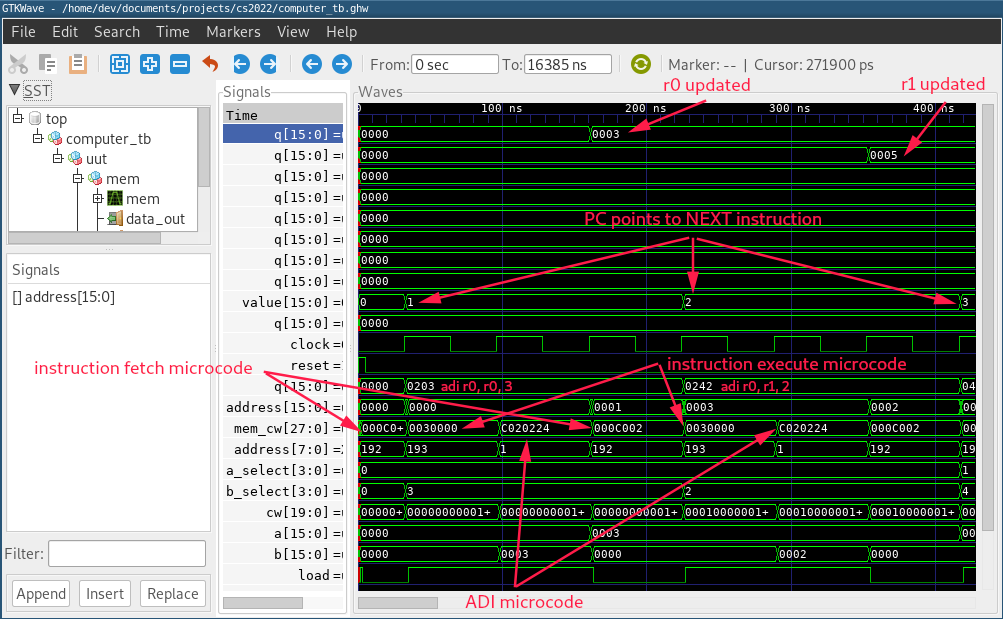
\includegraphics[width=\textwidth]{first_two}
	\caption{First two instructions}
\end{figure}

\newpage
\subsubsection{Up to first store}
The snippet below shows execution until the first \mi{c}{st} instruction. Red lines indicate which register 
changes correspond to which instructions and purple lines show the PC pointing to the next instruction to be 
executed.
\begin{figure}[h!]
	\centering
	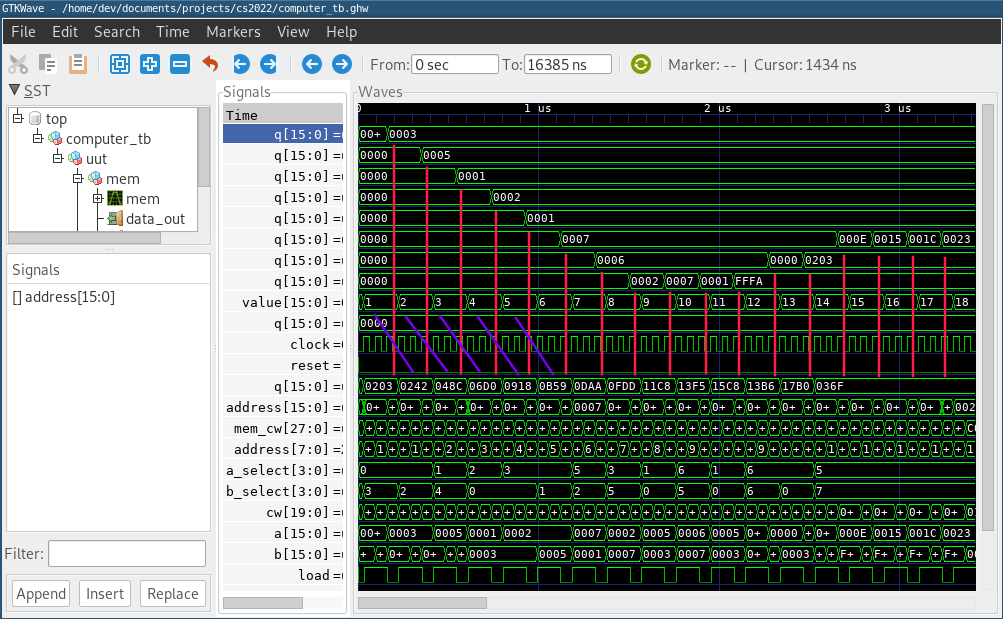
\includegraphics[width=\textwidth]{until_store}
	\caption{Execution up to the first store instruction}
\end{figure}

\newpage
\subsubsection{Storing and loading}
The snippet below shows execution of the store and load instructions. Note when the current main memory address 
changes from pointing to the next instruction being fetched to the pointer in \mi{c}{r5}.
\begin{figure}[h!]
	\centering
	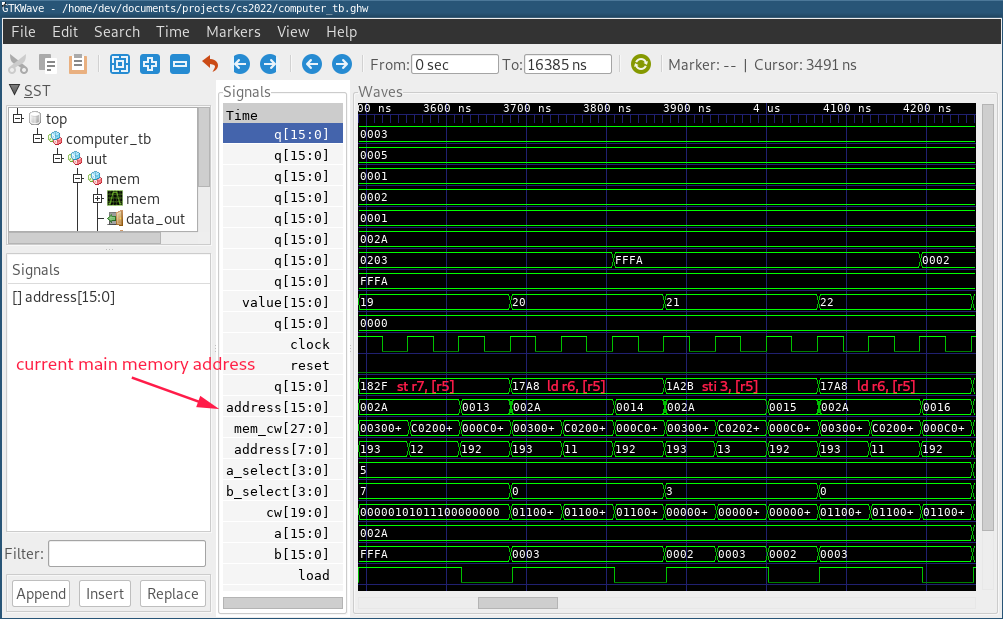
\includegraphics[width=\textwidth]{store_load}
	\caption{Load and store instructions}
\end{figure}

\newpage
\subsubsection{Shifting}
The snippet below shows a left shift by an immediate value. Note that the instruction takes numerous cycles to 
complete, running the microcode program for left shifts from above. The destination 
register holds a counter to keep track of how many shifts have been performed and the temporary register holds 
the shifted value. Once complete, this value is transferred back into the destination register.
\begin{figure}[h!]
	\centering
	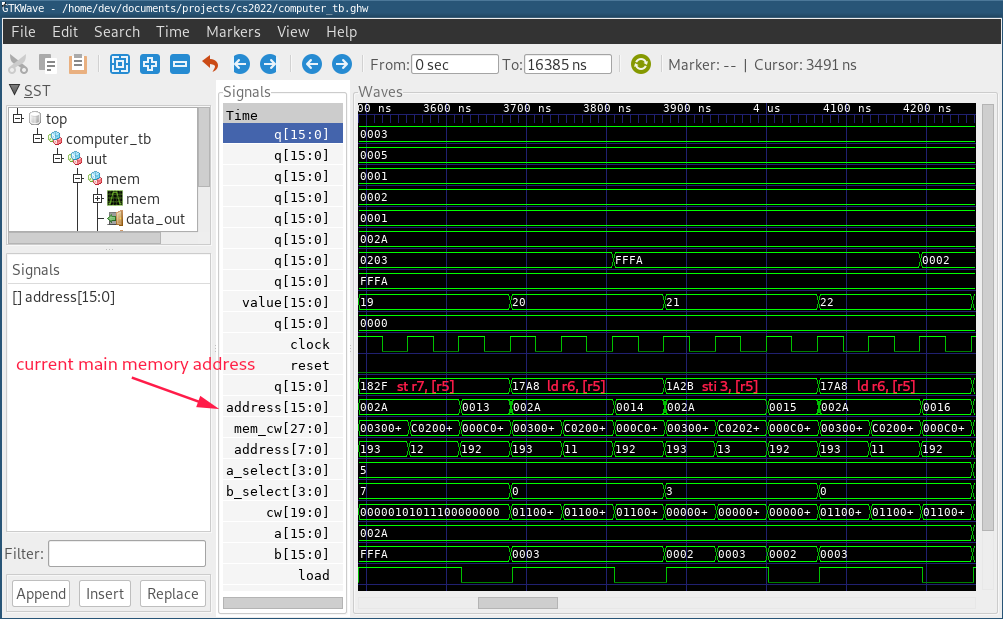
\includegraphics[width=\textwidth]{store_load}
	\caption{Load and store instructions}
\end{figure}

\newpage
\subsubsection{Unconditional branching}
The snippet below shows 3 unconditional branches. Note how the program counter changes according to the 
instructions instead of incrementing. See the sample program above and registers to see that instructions are 
skipped over by the branching.

Note also how the offsets are chosen since the PC always points to the instruction after the one currently 
executing.
\begin{figure}[h!]
	\centering
	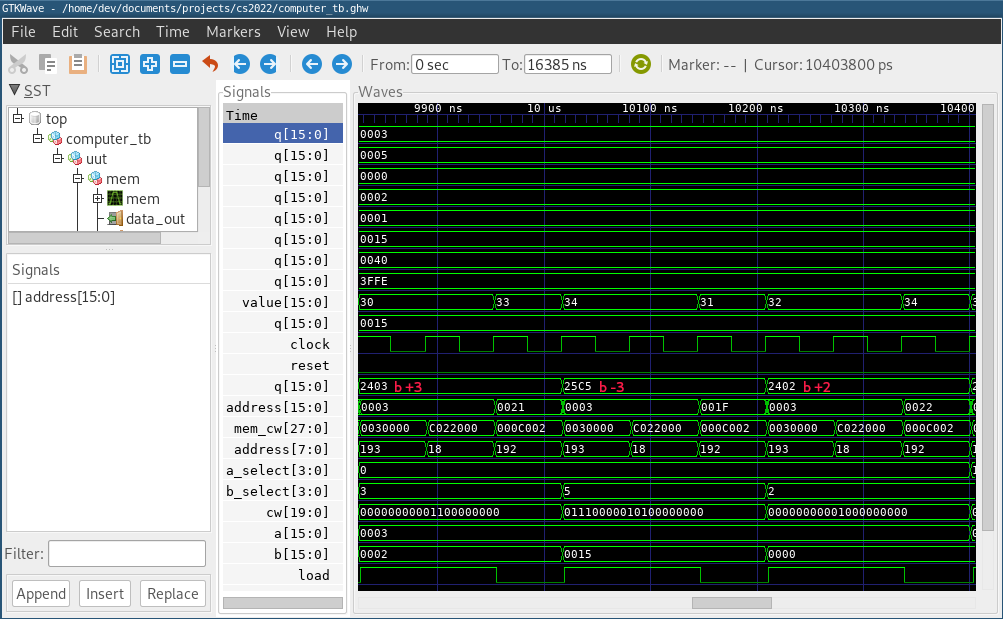
\includegraphics[width=\textwidth]{unc_branch}
	\caption{Unconditional branching}
\end{figure}

\newpage
\subsubsection{Conditional branching}
The snippet below shows a simple ``\mi{c}{for}-loop''. Notice the program repeatedly returns to the \mi{c}{BEQ} 
instruction until \mi{c}{r1} is \mi{c}{0}. At this point, execution continues (\mi{c}{adi r1, r1, 7} and two 
\mi{c}{NOP}'s) until halting at the end of the test program.

Note also how the \mi{c}{BEQ} takes longer to execute, as multiple microcode operations must execute to determine
whether the PC should be loaded with the provided offset or not.
\begin{figure}[h!]
	\centering
	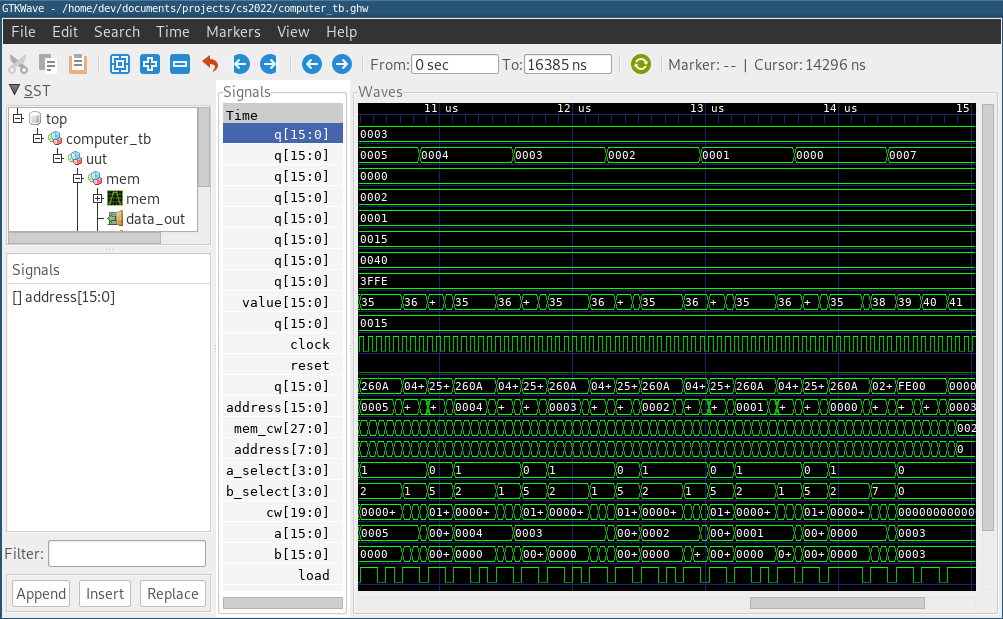
\includegraphics[width=\textwidth]{cond_branch}
	\caption{Conditional branching}
\end{figure}

\end{document}
# vim: nofoldenable
